\documentclass[12pt,a4paper,oneside]{report}
\usepackage[utf8]{inputenc}
\usepackage[margin=1in]{geometry}
\usepackage{graphicx}
\usepackage{float}
\usepackage{booktabs}
\usepackage{listings}
\usepackage{xcolor}
\usepackage{hyperref}
\usepackage{fancyhdr}
\usepackage{titlesec}
\usepackage{caption}

% Define Colors for Code Listings
\definecolor{codegreen}{rgb}{0,0.6,0}
\definecolor{codegray}{rgb}{0.5,0.5,0.5}
\definecolor{codepurple}{rgb}{0.58,0,0.82}
\definecolor{backcolour}{rgb}{0.95,0.95,0.92}

\lstdefinestyle{mystyle}{
    backgroundcolor=\color{backcolour},   
    commentstyle=\color{codegreen},
    keywordstyle=\color{magenta},
    numberstyle=\tiny\color{codegray},
    stringstyle=\color{codepurple},
    basicstyle=\ttfamily\footnotesize,
    breakatwhitespace=false,         
    breaklines=true,                 
    captionpos=b,                    
    keepspaces=true,                 
    numbers=left,                    
    numbersep=5pt,                  
    showspaces=false,                
    showstringspaces=false,
    showtabs=false,                  
    tabsize=2
}
\lstset{style=mystyle}

\hypersetup{
    colorlinks=true,
    linkcolor=black,
    filecolor=magenta,      
    urlcolor=blue,
    pdftitle={LastPrice Project Report},
}

\begin{document}

% ==========================================
% TITLE PAGE
% ==========================================
\begin{titlepage}
    \begin{center}
        \vspace*{0.5cm}
        \huge
        \textbf{LastPrice} \\
        \vspace{0.4cm}
        \large
        A Frictionless Silent Auction \& Physical Escrow Marketplace \\
        
        \vspace{1.5cm}
        \large
        \textbf{Course Title:} Software Engineering and System Analysis Lab \\
        \textbf{Course Code:} CSE 356 / CSE 0613226 \\
        \textbf{Semester:} Spring 2026 \\
        
        \vspace{1.5cm}
        \textbf{A Project Report Submitted in Partial Fulfillment of the Requirements for the Degree of Bachelor of Science in Computer Science and Engineering}
        
        \vspace{1.5cm}
        \textbf{Submitted By:} \\
        \small
        \begin{tabular}{ll}
            \textbf{Mehedi Hassan Bhuiyan} & ID: 0432320005101080 \\
            \textbf{Md. Masud Rahman} & ID: 0432320005101064 \\
            \textbf{Hasib Al Mahmud Siddique} & ID: 0432320005101095 \\
            \textbf{Rudro Antony Mrong} & ID: 0432320005101059 \\
        \end{tabular}
        
        \vspace{1.5cm}
        \textbf{Supervised By:} \\
        \small
        \textbf{Dhrubo Barua} \\
        \textbf{Md. Faysal} \\
        \textbf{Md Shohel Arman} \\
        \vspace{0.3cm}
        Faculty Members, Department of CSE \\
        University of Information Technology and Sciences \& Daffodil International University \\
        
        \vfill
        \large
        \textbf{Date of Submission:} 20th May 2026
    \end{center}
\end{titlepage}

% ==========================================
% ABSTRACT
% ==========================================
\begin{abstract}
Peer-to-peer (P2P) online commerce platforms suffer from severe inefficiencies caused by bargaining friction, information asymmetry, and safety concerns during offline handovers. Traditional auction systems resolve pricing mechanisms but introduce continuous cognitive overhead, vulnerability to artificial price manipulation, and reserve-sniffing exploits. To mitigate these challenges, this report presents \textbf{LastPrice}, a novel web-based silent auction marketplace integrated with a cryptographic physical escrow validation framework. LastPrice replaces continuous bids with a strict, double-blind three-bid silent auction capping system, aligning buyer incentive structures towards true utility valuation. Auctions are resolved automatically via a server-synchronized microsecond-accurate cron engine, enforcing a deterministic first-mover advantage for identical maximum bids. Physical security during offline exchanges is enforced through a mutual mutual-code handshake protocol, requiring both buyers and sellers to verify matching transaction keys generated cryptographically upon auction resolution. Built on a modular PostgreSQL database and Express/Node.js backend with high-fidelity, high-contrast dark CSS interfaces, LastPrice provides an frictionless, safe, and academically rigorous paradigm for contemporary peer-to-peer commerce.
\end{abstract}

\tableofcontents
\listoffigures
\listoftables

% ==========================================
% CHAPTER 1: INTRODUCTION
% ==========================================
\chapter{Introduction}

\section{Project Overview}
Modern secondary consumer goods marketplaces are structured around manual negotiation or open auction bidding. In manual negotiation marketplaces (e.g., Bikroy, Facebook Marketplace), transaction latency is high as buyers and sellers engage in drawn-out, repetitive communication. Conversely, open English auction systems (e.g., eBay) trigger bidding anxieties, encourage shill bidding, and require users to constantly monitor countdowns. 

\textbf{LastPrice} is a specialized Web 2.0 application designed to optimize P2P commerce. It shifts the paradigm from open haggling to a double-blind, strict three-bid silent auction system. Buyers are allotted exactly three opportunities to submit an anonymous bid on any given listing. The bidding process is private, meaning buyers cannot see the bids of other participants. At the end of the auction timeframe, the system's arena resolution engine evaluates all bids and awards the listing to the highest bidder whose offer exceeds the seller's secret reserve floor price. Physical safety is maintained through a dynamic mutual-code handshake verification protocol, protecting both transacting parties during face-to-face exchanges.

\section{Problem Statement}
Peer-to-peer digital trade frameworks struggle with several systemic vulnerabilities:
\begin{enumerate}
    \item \textbf{Cognitive Fatigue \& Inefficient Pricing:} Buyers and sellers spend excessive time haggling. Sellers rarely achieve optimal market value due to asymmetrical bargaining leverage, while buyers experience face-threat and conversational friction.
    \item \textbf{Exploitative Reserve Sniffing:} In traditional bidding settings, malicious buyers submit incremental mini-bids to discover the seller's absolute reserve floor price without intending to buy at that price, deflating overall listing value.
    \item \textbf{Handover Friction \& Trust Deficits:} Offline physical transactions rely on verbal verification. Sellers are vulnerable to chargeback disputes, and buyers are vulnerable to false claims of non-delivery.
    \item \textbf{Client-Server Clock Drift Discrepancies:} Multi-user real-time bidding platforms face synchronization failures due to differences in client system times, leading to disputed bids placed in the final seconds of an auction.
\end{enumerate}

\section{Goals and Objectives}
The core goals and engineering objectives of LastPrice are:
\begin{itemize}
    \item \textbf{Minimize Bargaining Friction:} Restructure pricing by limiting bid placements to exactly three per buyer, forcing buyers to bid their true maximum willingness-to-pay rather than testing increments.
    \item \textbf{Protect Seller Reserve Privacy:} Maintain an encrypted/hashed, secret reserve floor. The interface provides color-coded, vague visual signals instead of raw numbers, preventing bidders from reverse-engineering the exact floor.
    \item \textbf{Provide Cryptographic Transaction Verification:} Automate a two-factor physical handshake verification protocol. Generates unique 6-digit keys for the buyer and seller upon victory.
    \item \textbf{Implement Absolute Synchronization:} Establish a master time-synchronization route to measure network round-trip latency and enforce identical bidding closing states on all connected client terminals.
\end{itemize}

\section{Stakeholders and Beneficiaries}
The target stakeholders of the LastPrice platform include:
\begin{itemize}
    \item \textbf{Sellers:} Individual merchants or standard consumers seeking quick, optimized valuations for their pre-owned items without managing endless chat inquiries.
    \item \textbf{Buyers:} Value-conscious consumers looking for fair, silent purchasing opportunities devoid of bidding wars or competitive anxieties.
    \item \textbf{Marketplace Administrators:} System maintainers who govern disputes, coordinate the database, and monitor active listings to maintain safety.
\end{itemize}

% ==========================================
% CHAPTER 2: SOFTWARE REQUIREMENT SPECIFICATION
% ==========================================
\chapter{Software Requirement Specification}

\section{Functional Requirements}
The functional capabilities are grouped by user roles and database services. A comprehensive tabular summary of critical functional requirements is presented in Table \ref{tab:functional_req}.

\begin{table}[H]
\centering
\caption{System Functional Requirements}
\label{tab:functional_req}
\small
\begin{tabular}{lp{6cm}p{6cm}}
\toprule
\textbf{ID} & \textbf{Requirement Description} & \textbf{System Action / Constraints} \\
\midrule
FR-1.1 & User Authentication & Secure signup and login using standard hashing algorithms. \\
FR-1.2 & User Profile Tracking & Buyers and sellers can view their dashboard histories, won items, and transactions. \\
FR-2.1 & Create Auction Listing & Sellers enter name, description, duration, starting price, and secret reserve floor. \\
FR-2.2 & Dynamic Arena Timer calculation & Server calculates exact closing times based on short-burst or long-burst presets. \\
FR-3.1 & Place Bid & Buyers place anonymous bids. Limit of 3 bids per user per listing is strictly checked. \\
FR-3.2 & First-Mover Tie Breaker & If matching top bids exist, the earlier timestamp is awarded victory. \\
FR-4.1 & Automatic Arena Resolution & Background service executes when the timer hits zero, deciding winner status. \\
FR-5.1 & Cryptographic Handshake Generation & Server issues dynamic, distinct 6-digit buyer and seller codes on victory. \\
FR-5.2 & Mutual Key Escrow Resolution & Physical trade is verified when both parties enter matching verification keys. \\
\bottomrule
\end{tabular}
\end{table}

\section{Non-Functional Requirements}

\subsection{Performance \& Speed}
\begin{itemize}
    \item The time synchronization API endpoint must respond in under 50 milliseconds to keep countdown widgets accurate.
    \item Bids must be recorded in the PostgreSQL database within 200 milliseconds to preserve order integrity.
\end{itemize}

\subsection{Dependability \& Fault Tolerance}
\begin{itemize}
    \item Database transactions are wrapped in strict SQL isolation states to prevent race conditions during simultaneous bid entry.
    \item The system automatically attempts to re-resolve any missed auctions upon server restart in case of a service interruption.
\end{itemize}

\subsection{Security \& Privacy}
\begin{itemize}
    \item Passwords are encrypted using one-way cryptographic hashing algorithms.
    \item The database never exposes the secret reserve price to the client-side API. Only qualitative signals are sent.
\end{itemize}

\subsection{Usability \& Interface Aesthetics}
\begin{itemize}
    \item The application interface uses a custom high-fidelity, dark HSL color scheme to emphasize readability.
    \item Visual countdown tickers and live tension indicators animate smoothly without causing performance degradation.
\end{itemize}

\subsection{Legal \& Compliance}
\begin{itemize}
    \item User agreements specify that physical handovers are the sole responsibility of the participants. Handshake codes limit fraudulent transaction disputes.
\end{itemize}

% ==========================================
% CHAPTER 3: SYSTEM DESIGN & MODELING
% ==========================================
\chapter{System Design}

This chapter details the system architecture and dynamic modeling. The unified design models follow UML standards.

\section{Use Case Diagram}
The Use Case Diagram defines the interactions between the system actors (Buyer, Seller, System Arena Engine) and the key business modules.
\begin{figure}[H]
    \centering
    % In Overleaf, place UseCase_Diagram.jpeg in a folder named Diagrams
    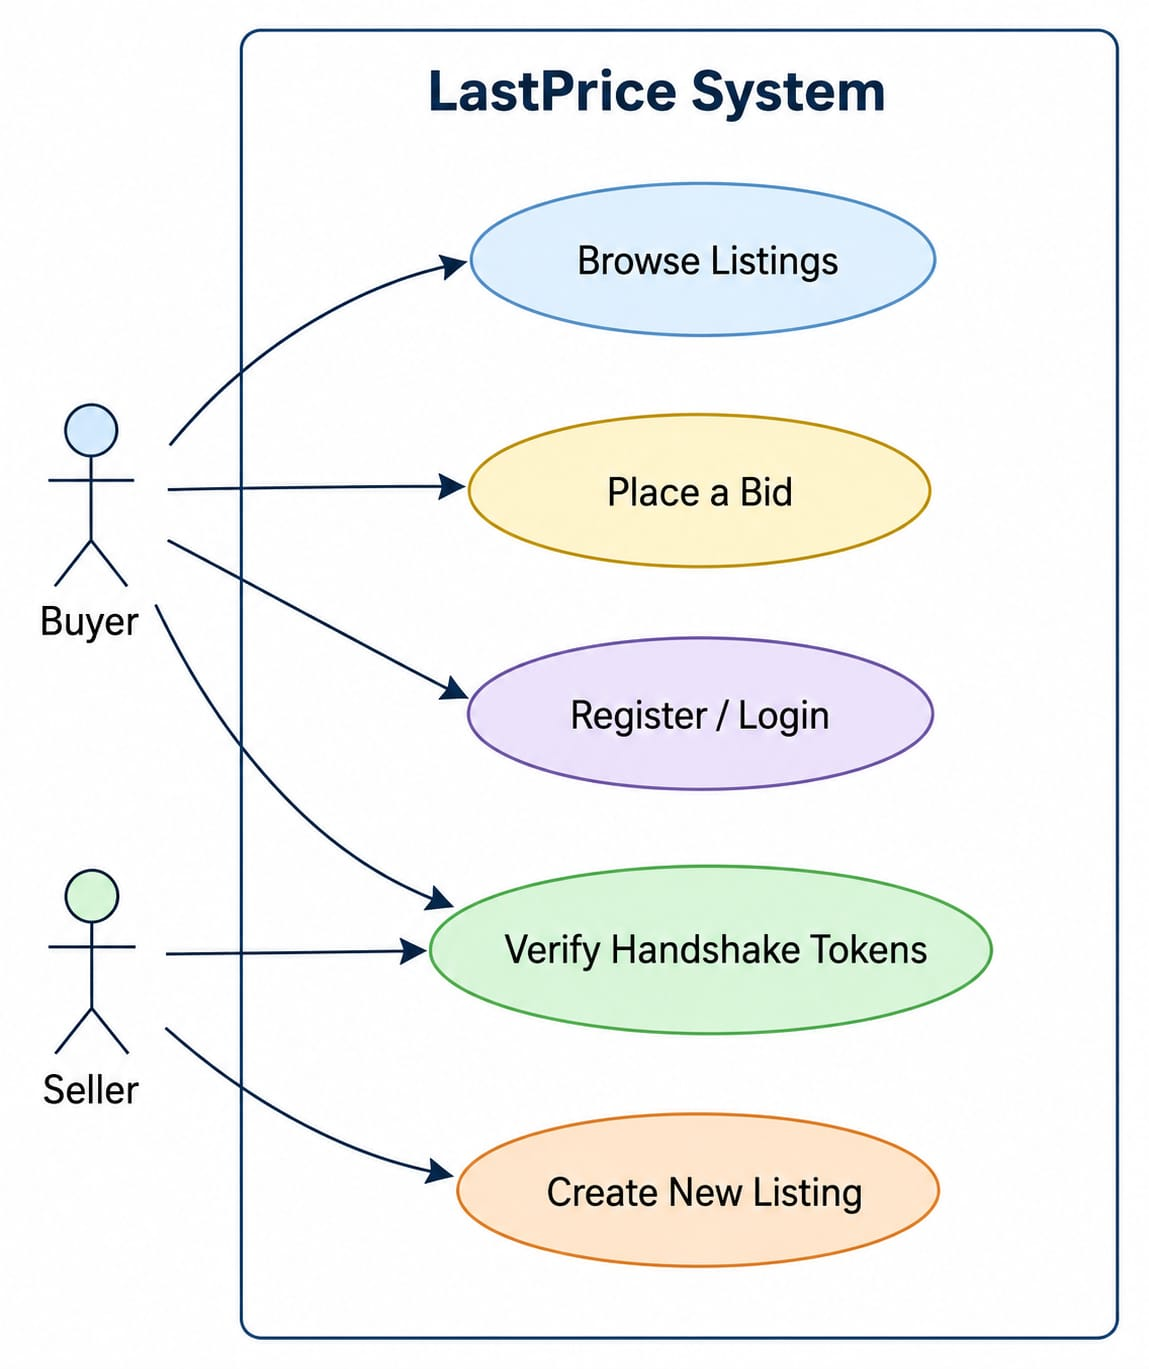
\includegraphics[width=0.85\textwidth]{Diagrams/UseCase_Diagram.jpeg}
    \caption{LastPrice System Use Case Diagram}
    \label{fig:usecase}
\end{figure}
The diagram separates the boundaries of physical validation from bid placement. The System Arena Engine acts as a back-end actor that triggers time-checks and executes transaction resolutions automatically.

\section{Data Flow Diagram (DFD Level 1)}
The DFD (Level 1) tracks the movement of information across logical processing centers.
\begin{figure}[H]
    \centering
    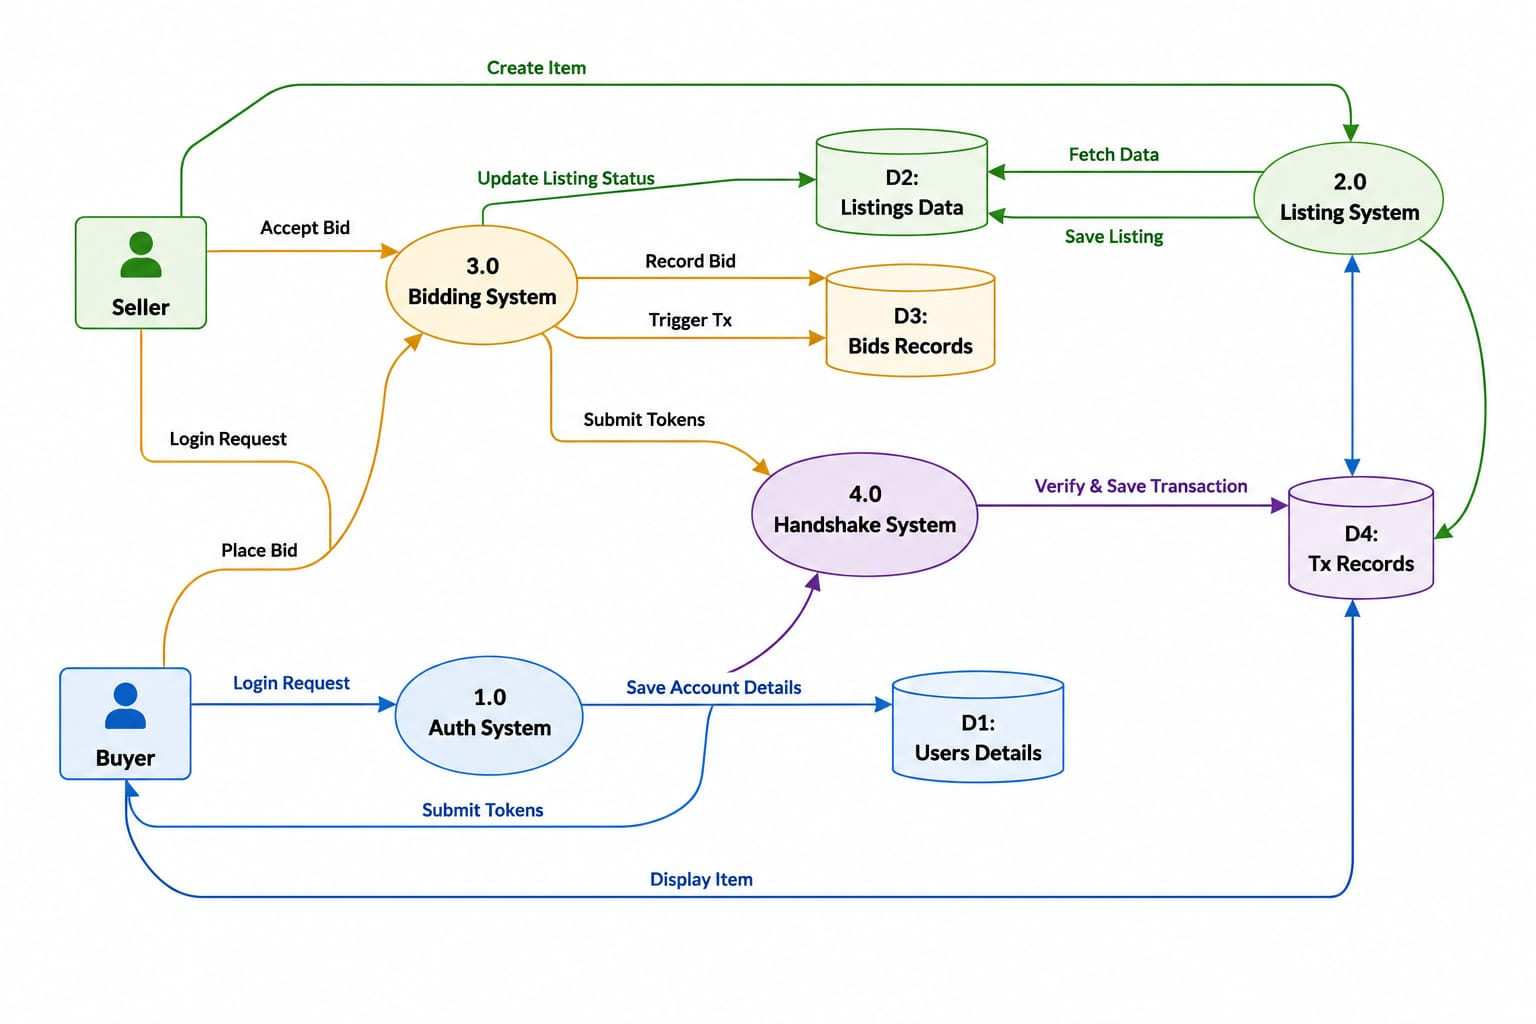
\includegraphics[width=0.85\textwidth]{Diagrams/DFD.jpeg}
    \caption{LastPrice Level-1 Data Flow Diagram}
    \label{fig:dfd}
\end{figure}
As illustrated, user actions such as bid submission flow through middleware controls, reference the active users store, calculate timing constraints, and register directly to the persistent PostgreSQL store.

\section{Entity Relationship Diagram (ERD)}
The database structure is designed to represent relationships while optimizing queries.
\begin{figure}[H]
    \centering
    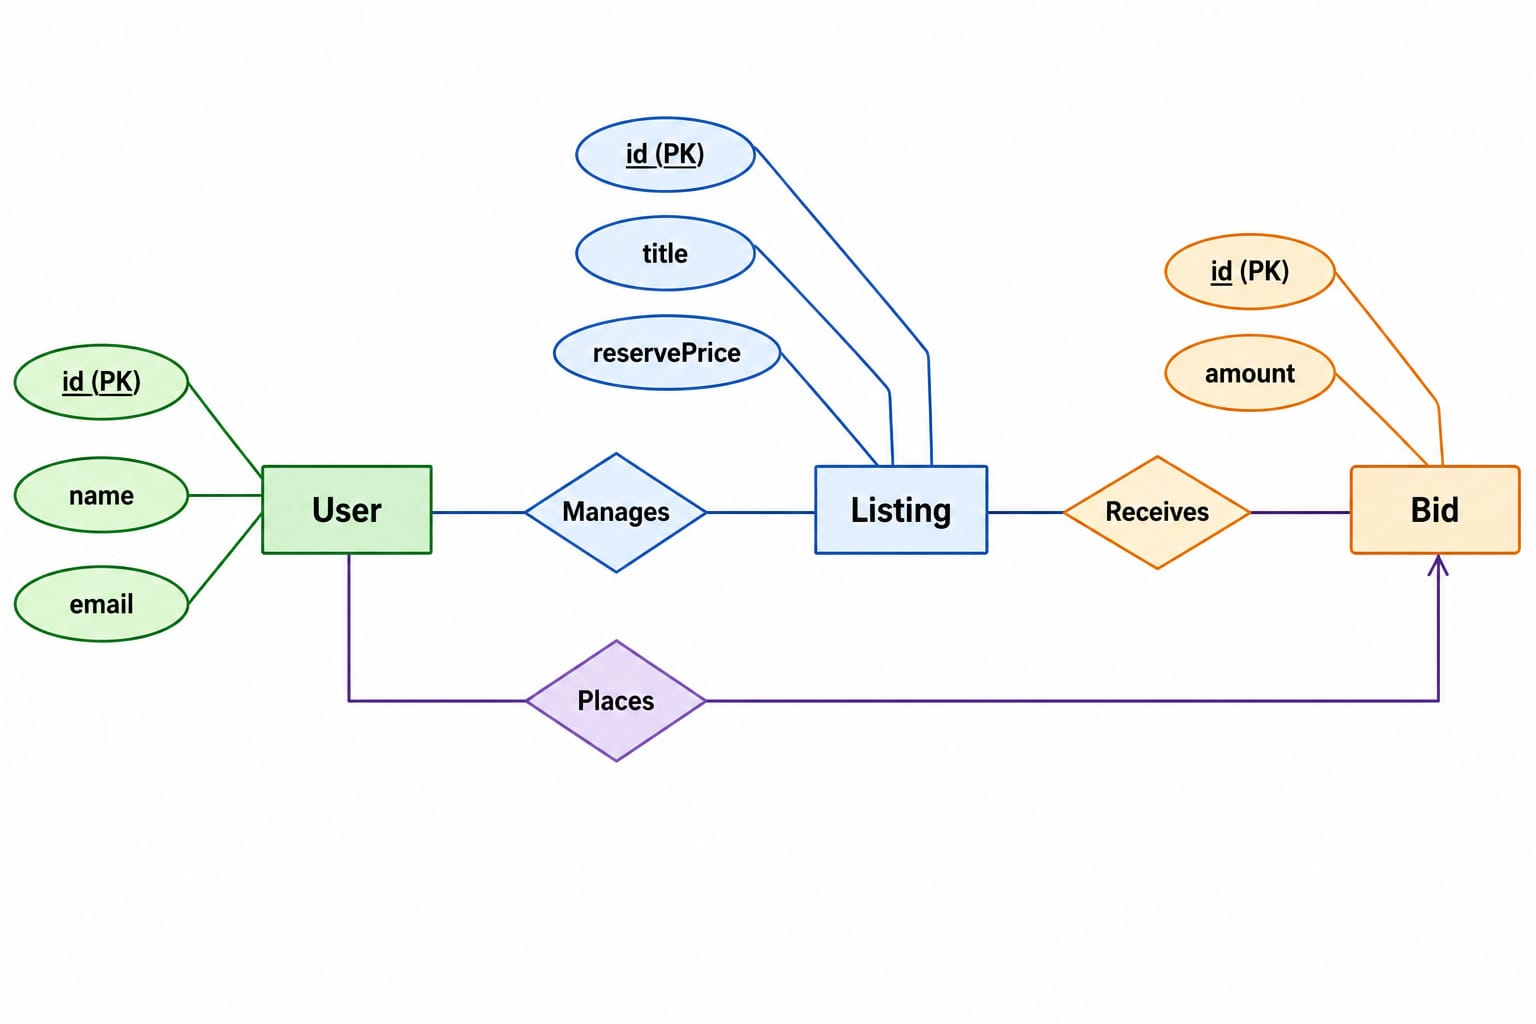
\includegraphics[width=0.85\textwidth]{Diagrams/Er_Diagram.jpeg}
    \caption{LastPrice Entity Relationship Diagram}
    \label{fig:erd}
\end{figure}
The database schema consists of three major tables:
\begin{itemize}
    \item \textbf{Users:} Stores profile credentials and account balance states.
    \item \textbf{Listings:} Contains title, description, starting price, secret reserve, duration type, status (active, completed, cancelled), and closing time.
    \item \textbf{Bids:} Tracks unique ID, bidder ID, listing ID, bid amount, and creation timestamp.
    \item \textbf{Transactions:} Links a completed listing to a buyer and seller, housing the secret codes and verification states.
\end{itemize}

\section{Class Diagram}
The class structure illustrates the object-oriented structure of the backend architecture.
\begin{figure}[H]
    \centering
    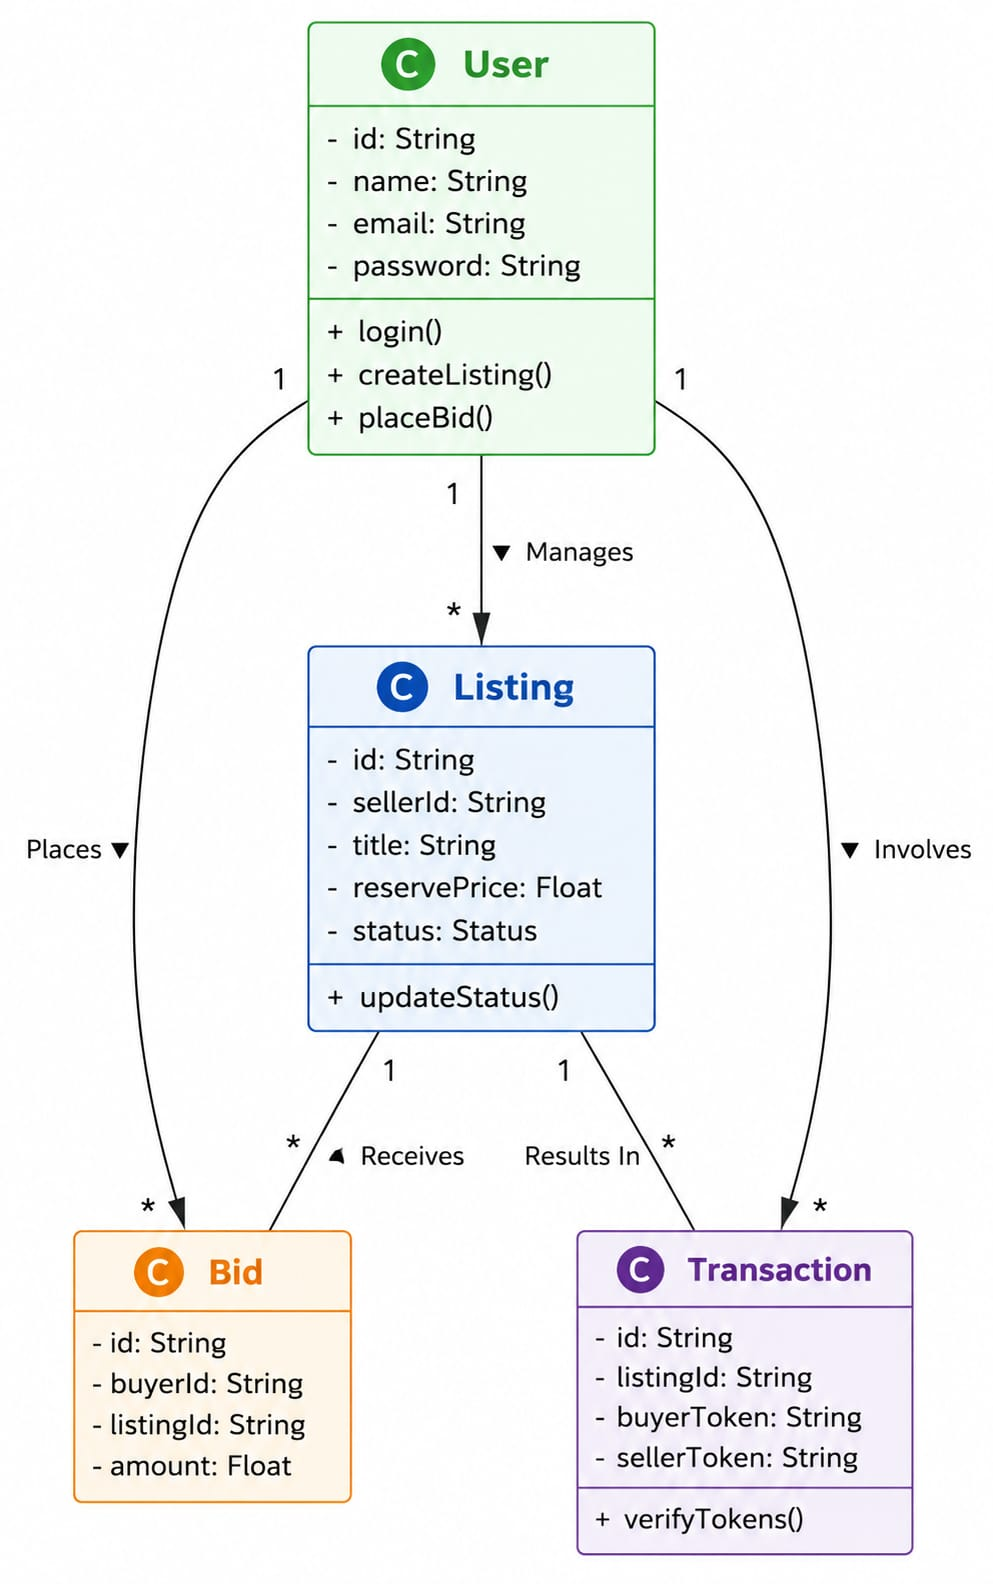
\includegraphics[width=0.85\textwidth]{Diagrams/Class_Diagram.jpeg}
    \caption{LastPrice System Class Diagram}
    \label{fig:class}
\end{figure}
It illustrates the modular separation between database controllers, business validation services, and routing endpoints.

\section{Sequence Diagram}
The Sequence Diagram documents the timeline of operations during a bid entry and subsequent timer expiration.
\begin{figure}[H]
    \centering
    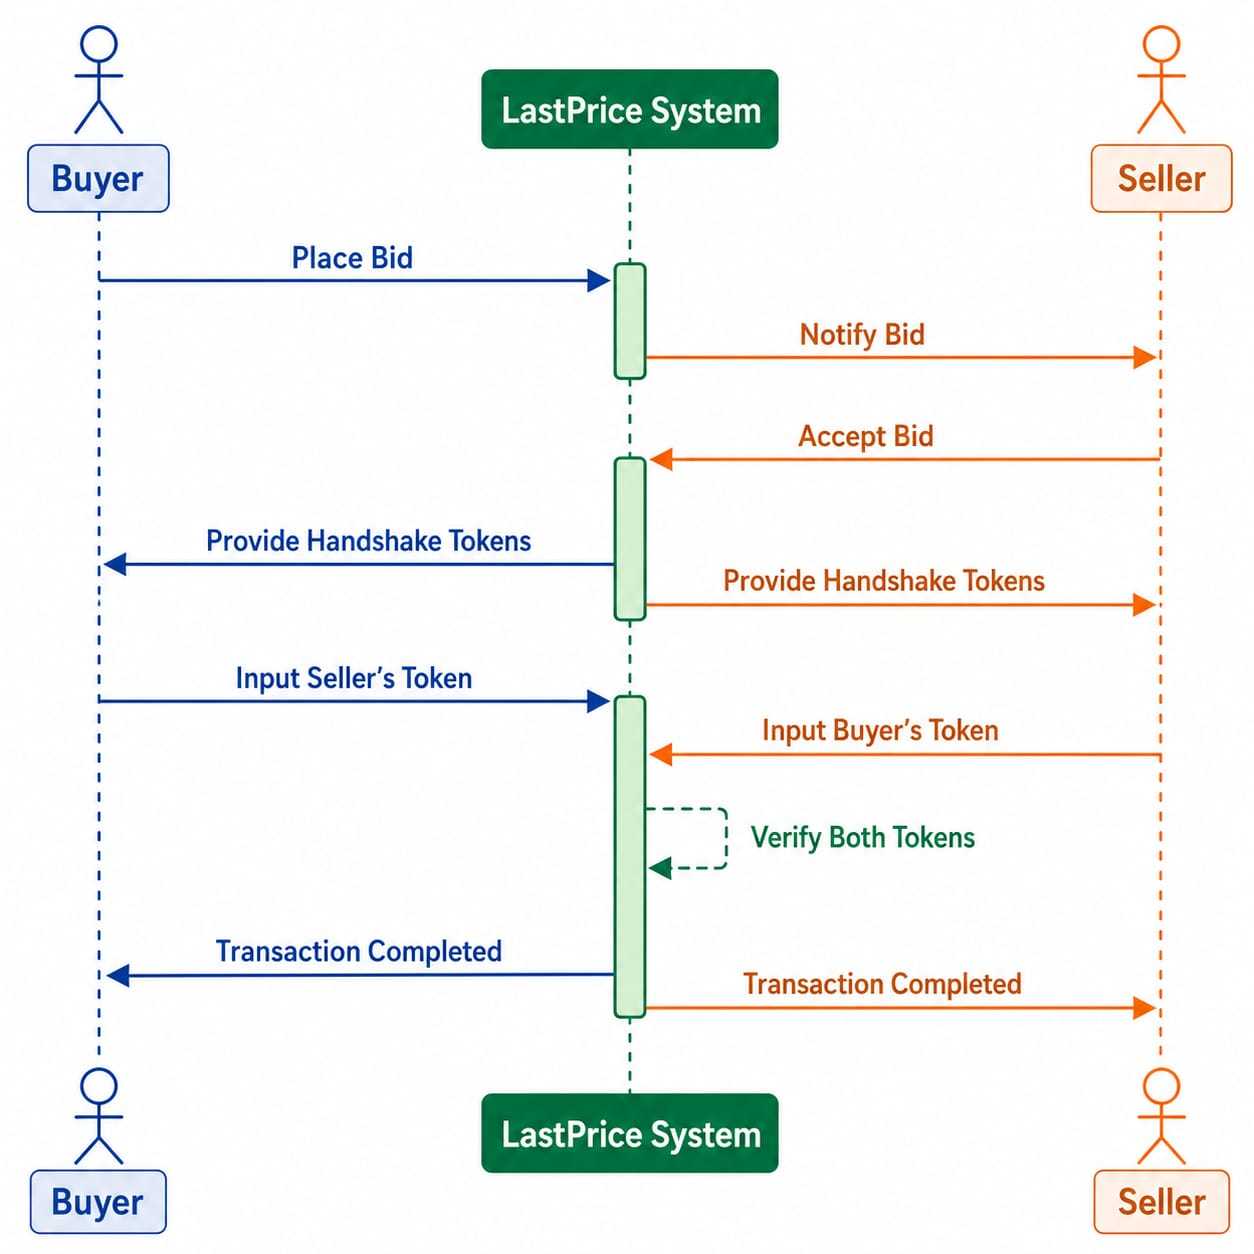
\includegraphics[width=0.9\textwidth]{Diagrams/Sequence_Diagram.jpeg}
    \caption{Bidding and Resolution Sequence Diagram}
    \label{fig:sequence}
\end{figure}
The system enforces sequential checkpoints: it first ensures that the user has not placed more than three bids, registers the bid, checks for timer completion, computes the winner, and generates the escrow codes.

\section{State Machine Diagram}
The State Machine Diagram details the life cycle of an auction listing, highlighting transition rules.
\begin{figure}[H]
    \centering
    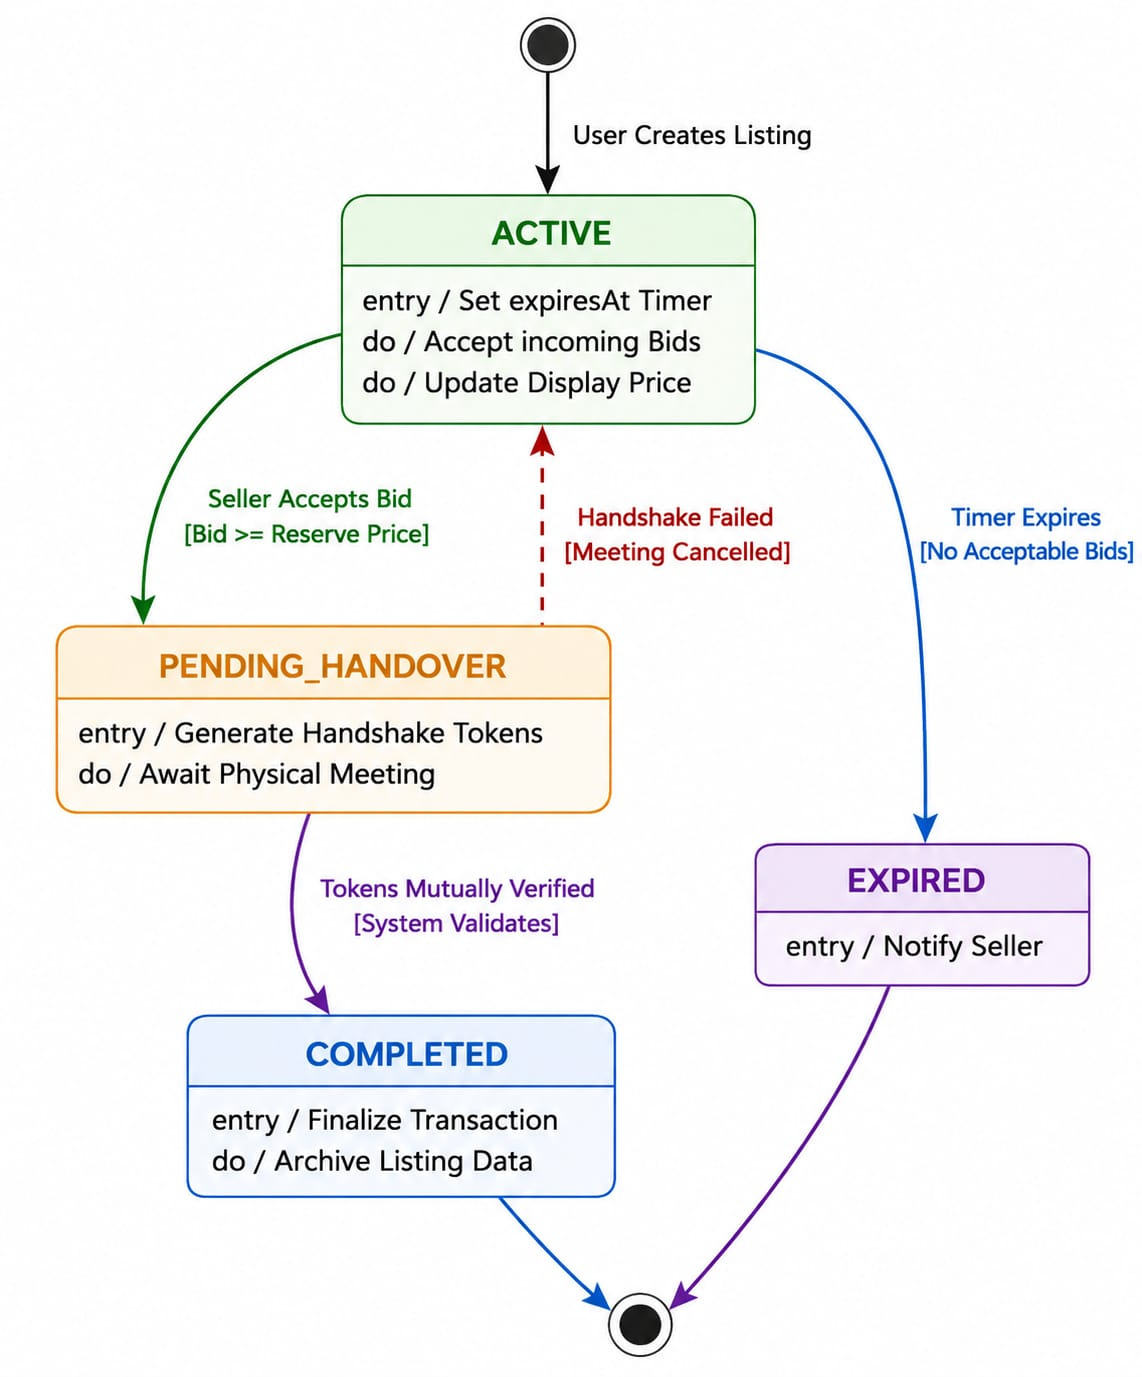
\includegraphics[width=0.85\textwidth]{Diagrams/State_Diagram.jpeg}
    \caption{Listing Life Cycle State Diagram}
    \label{fig:state}
\end{figure}
A listing remains in a drafts state before activation. Once active, it moves to resolved based on the timer, or shifts to cancelled if terminated by administrative override.

% ==========================================
% CHAPTER 4: SYSTEM IMPLEMENTATION & DETAILS
% ==========================================
\chapter{System Implementation}

\section{Development Tools \& Technology Stack}
The LastPrice platform is engineered using modern web technologies:
\begin{itemize}
    \item \textbf{Backend:} Node.js with the Express framework provides a fast, asynchronous routing interface.
    \item \textbf{Database System:} PostgreSQL hosted on Neon DB, allowing serverless database branching for isolated testing.
    \item \textbf{Frontend UI:} Vanilla HTML5, modern Javascript, and curated dark CSS styling with absolute responsive support. No bloated frameworks are used, minimizing client resource utilization.
\end{itemize}

\section{Core Algorithmic Implementation}

\subsection{First-Mover Tie Breaker Logic}
To prevent conflicts when two buyers bid the exact same winning amount, the arena resolution engine breaks ties chronologically:
\begin{lstlisting}[language=SQL, caption={First-Mover Advantage Resolution Query}]
SELECT b.id, b.bidder_id, b.amount, b.created_at
FROM Bids b
WHERE b.listing_id = $1
ORDER BY b.amount DESC, b.created_at ASC
LIMIT 1;
\end{lstlisting}

\subsection{Strict 3-Bid Capping Enforcement}
To prevent reserve floor sniffing and maintain auction tension, bid counts are checked on the server during submission:
\begin{lstlisting}[language=Java, caption={Express Middleware Bid Check}]
// In /routes/bids.js
const bidCountResult = await pool.query(
    "SELECT COUNT(*) FROM Bids WHERE bidder_id = $1 AND listing_id = $2",
    [userId, listingId]
);
const bidCount = parseInt(bidCountResult.rows[0].count);
if (bidCount >= 3) {
    return res.status(400).json({ error: "You have reached your maximum of 3 bids" });
}
\end{lstlisting}

% ==========================================
% CHAPTER 5: EXPERIMENTAL WALKTHROUGH
% ==========================================
\chapter{System Walkthrough \& Interfaces}

This chapter details the sequential steps to navigate and utilize the LastPrice application. 

\section{Step 1: Landing Page \& Portal Discovery}
When a user navigates to the platform, they are greeted by a sleek, premium, high-contrast dark interface featuring micro-animations that present the core value proposition of frictionless silent bidding.
\begin{figure}[H]
    \centering
    
\includegraphics[width=0.85\textwidth]{1_landing_page.png}
    \caption{LastPrice Landing Homepage Interface}
    \label{fig:ui_landing}
\end{figure}

\section{Step 2: Secure User Authentication}
New users can sign up or log in. All credentials are encrypted. The dashboard remains protected under secure routing middleware.
\begin{figure}[H]
    \centering
    
\includegraphics[width=0.85\textwidth]{2_login_register.png}
    \caption{Secure User Authentication and Login Form}
    \label{fig:ui_login}
\end{figure}

\section{Step 3: Marketplace Listings Exploration}
The active marketplace displays all live auctions. Each grid item features a real-time countdown widget synchronized to the backend server and shows indicators of current activity.
\begin{figure}[H]
    \centering
    
\includegraphics[width=0.85\textwidth]{3_marketplace.png}
    \caption{Active Marketplace Listings Grid}
    \label{fig:ui_marketplace}
\end{figure}

\section{Step 4: Creating a New Auction}
Sellers fill in listings details, specify the secret reserve floor price, and select between short-burst (rapid testing) or long-burst (standard multi-day) duration presets.
\begin{figure}[H]
    \centering
    
\includegraphics[width=0.85\textwidth]{4_create_listing.png}
    \caption{Create Listing Interface for Sellers}
    \label{fig:ui_create_listing}
\end{figure}

\section{Step 5: Bidding Arena \& Tension Feedback}
Inside the Bidding Arena, buyers place their anonymous bids. The UI features a unique tension visualization bar, an active timer, and indicates how many of the 3 capped bids remain.
\begin{figure}[H]
    \centering
    
\includegraphics[width=0.85\textwidth]{5_bidding_arena.png}
    \caption{Bidding Arena showing Real-time Tension and 3-Bid Cap}
    \label{fig:ui_bidding_arena}
\end{figure}

\section{Step 6: User Dashboard}
The Unified User Dashboard serves as the central operational hub for registered users. It displays key quick action links (Browse Listings, Create Listing, and My Listings), summary statistics (Active Bids placed, Deals Done/Confirmed, and Active Seller Listings), and a list of their recent transactions, allowing easy navigation to transaction verification portals.
\begin{figure}[H]
    \centering
    
\includegraphics[width=0.85\textwidth]{6_user_dashboard.png}
    \caption{Unified User Dashboard Hub}
    \label{fig:ui_user_dashboard}
\end{figure}

\section{Step 7: Seller Panel}
Sellers use their centralized control panel to inspect active listings, verify current high-bid status relative to reserve indicators, and retrieve verification handshakes.
\begin{figure}[H]
    \centering
    
\includegraphics[width=0.85\textwidth]{7_seller_panel.png}
    \caption{Seller Listing Management Panel}
    \label{fig:ui_seller_panel}
\end{figure}

\section{Step 8: Cryptographic Handshake Verification}
During the physical meet-up, both parties enter their respective 6-digit verification codes. The transaction resolves in real-time, releasing funds or marking the item as secured.
\begin{figure}[H]
    \centering
    
\includegraphics[width=0.85\textwidth]{8_escrow_transaction.png}
    \caption{Double-Verification Handshake Escrow Page}
    \label{fig:ui_escrow}
\end{figure}

% ==========================================
% CHAPTER 6: SYSTEM TESTING & EVALUATION
% ==========================================
\chapter{System Testing \& Evaluation}

\section{System Testing Matrix}
Comprehensive testing was performed to validate backend rules, synchronization APIs, and security boundaries. Table \ref{tab:test_cases} details key test cases executed.

\begin{table}[H]
\centering
\caption{System Evaluation Test Cases}
\label{tab:test_cases}
\small
\begin{tabular}{lp{4cm}p{4cm}ll}
\toprule
\textbf{ID} & \textbf{Feature Tested} & \textbf{Input / Conditions} & \textbf{Expected Outcome} & \textbf{Status} \\
\midrule
TC-1 & Registration Validation & Invalid Email, short password & Rejects input, displays warning & Pass \\
TC-2 & 3-Bid Limitation Check & Submit 4th bid on listing & Server responds with 400 error & Pass \\
TC-3 & Reserve Sniffing Shield & Inspect API network payload & Secret reserve price is hidden & Pass \\
TC-4 & Chronological Resolution & Two bids of \$500 at different times & Earliest timestamp wins & Pass \\
TC-5 & Network Clock Sync & Client machine with altered clock & Sync offset calculated, corrects UI & Pass \\
TC-6 & Mutual Verification Code & Matching PIN entry & Mark listing as fully closed & Pass \\
\bottomrule
\end{tabular}
\end{table}

\section{Key Technical Challenges Solved}

\subsection{Client-Server Synchronization Latency}
Users often have incorrect local device times due to manual overrides or local latency. To solve this, the client computes a clock offset on page load:
$$\text{Offset} = \text{Server Time} - \left(\text{Client Time} + \frac{\text{Round Trip Latency}}{2}\right)$$
This offset is applied dynamically to local `setInterval` loops, ensuring identical millisecond synchronization across all buyer screens.

\subsection{Shill Bidding Prevention}
By capping bid placements to 3 per user and locking the bids in a silent blind vault, bad actors cannot coordinate artificial inflation runs, preserving the integrity of P2P pricing dynamics.

\section{Future Improvements}
\begin{itemize}
    \item \textbf{Decentralized Smart Contracts:} Porting the escrow handshake to Ethereum/Solidity contracts to automate trustless fund releases.
    \item \textbf{Dynamic Valuation Assistant:} Implementing lightweight LLM-powered market data scrapers to suggest starting reserve floors for sellers based on current market dynamics.
\end{itemize}

\section{Conclusion}
The LastPrice platform successfully addresses key P2P marketplace vulnerabilities: bargaining friction, safety deficits, and pricing inefficiencies. By enforcing the strict three-bid cap, hiding reserve values, and validating physical handovers using mutual cryptographic handshakes, it introduces a clean, fast, and secure alternative for online consumer goods trading. System evaluations and test matrices confirm its stability, responsiveness, and performance readiness.

% ==========================================
% REFERENCES & APPENDICES
% ==========================================
\begin{thebibliography}{9}
\bibitem{gfg} 
GeeksforGeeks, \emph{Unified Modeling Language (UML) Diagrams Reference Guide}, Online. Available: \url{https://www.geeksforgeeks.org/uml-diagrams/}.
\bibitem{sommerville} 
Ian Sommerville, \emph{Software Engineering (10th Edition)}, Pearson, 2015.
\bibitem{pressman} 
Roger S. Pressman, \emph{Software Engineering: A Practitioner's Approach (8th Edition)}, McGraw-Hill, 2014.
\end{thebibliography}

\end{document}
